\documentclass{article}

\usepackage{enumitem}
\usepackage{listings}
\usepackage{color}
\usepackage{amsmath}
\usepackage{hyperref}
\usepackage{graphicx}
\usepackage{pgffor}
\usepackage{xparse}
\usepackage{expl3}
\usepackage{tabularx, makecell}
\usepackage{multirow}
\usepackage{booktabs}
\usepackage{indentfirst}
\usepackage{lipsum}
\usepackage{sectsty}
\usepackage[utf8]{inputenc}
\usepackage{csquotes}
\usepackage{xcolor}
\usepackage{fancyvrb}
\usepackage{fancyhdr}
\usepackage{fancyvrb}
\usepackage[most]{tcolorbox}
\usepackage{blindtext}
\usepackage{caption}
\usepackage{etoolbox}
\usepackage{booktabs}
\usepackage{karnaugh-map}
\usepackage{tikz}
\usepackage{mdframed}
\usepackage{calc}
\usepackage[nomessages]{fp}
\usepackage{pgfplots}

\graphicspath{{./}}

\definecolor{codegreen}{rgb}{0,0.6,0}
\definecolor{codegray}{rgb}{0.5,0.5,0.5}
\definecolor{codepurple}{rgb}{0.58,0,0.82}
\definecolor{backcolour}{rgb}{0.95,0.95,0.92}

\sectionfont{\bfseries\Large\center} 

% Lstlisting configuartions for C++
\lstset{
	language=C++,
	frame=single,
	rulecolor=\color{gray},
	basicstyle=\fontsize{5}{5}\ttfamily,
	keywordstyle=\color{blue},
	stringstyle=\color{orange},
	commentstyle=\color{gray},
	extendedchars=true,
	keepspaces=true,
	numbers=left,
	numbersep=5pt,
	numberstyle=\color{gray},
	tabsize=4,
	morecomment=[l][\color{gray}]{\#}
}

% Lstlisting configuartions for algorithm code
\newcounter{nalg}[section]
\renewcommand{\thenalg}{\arabic{nalg}}
\DeclareCaptionLabelFormat{algocaption}{\textbf{Algorithm \thenalg}}
\lstnewenvironment{algorithm}[1][]
{
    \refstepcounter{nalg}
    \captionsetup{labelformat=algocaption,labelsep=colon}
    \lstset{
        mathescape=true,
        frame=tB,
        numbers=left, 
        numberstyle=\tiny,
        basicstyle=\scriptsize, 
        keywordstyle=\color{blue}\bfseries\em,
        keywords={,input, output, return, datatype, function, in, if, else, foreach, while, begin, end, then, }
        numbers=left,
        xleftmargin=.04\textwidth,
        #1
    }
}{}

\pgfplotsset{compat=1.13}

\begin{document}
	% Vars
	\newcommand{\ROne}{99.8}
	\newcommand{\RTwo}{198}
	\newcommand{\RThree}{53.7}
	\newcommand{\RMax}{473}
	
	\newcommand{\IPosOne}{42.1}
	\newcommand{\IPosTwo}{96.0}

	\newcommand{\UExOneOne}{4.24}
	\newcommand{\UExOneTwo}{8.43}
	\newcommand{\UExOneThree}{2.26}

	\newcommand{\IExTwoOne}{61.7}
	\newcommand{\IExTwoTwo}{43.2}
	\newcommand{\IExTwoThree}{18.6}

	\newcommand{\UExTwoOne}{6.66}
	\newcommand{\UExTwoTwo}{8.69}
	\newcommand{\UExTwoThree}{8.69}

	% <Square cases>
	\makeatletter
	\newenvironment{sqcases} {
		\matrix@check\sqcases\env@sqcases
	}{
		\endarray \right.
	}
	\def\env@sqcases {
		\let \@ifnextchar \new@ifnextchar
		\left \lbrack
		\def \arraystretch{1.2}
		\array{@{}l@{\quad}l@{}}
	}
	\makeatother
	% </Square cases>

	% Begin of the document

	\title{CDE laboratory\_01}
	\author{Terman Emil FAF161}
	\maketitle

	% Write at bottom
	\vspace*{\fill}
	
	\centering
	
\includegraphics{imgs/UTM_logo.png}

	\begin{flushright}
		Prof: O. Lupan
	\end{flushright}

	\LaTeX
	\pagebreak %-----------------------------------------------End of title page

	\raggedright
	\section{Verificarea îndeplinirii legilor lui Ohm si Kirchhoff pentru circuitele electrice neramificate si ramificate.}
		\begin{center}
			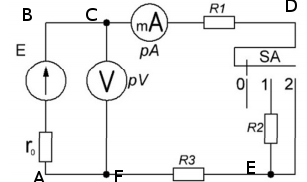
\includegraphics[scale=0.7]{./imgs/ElectricCircuit1.jpg}
		\end{center}

	\subsection{}
		\[
			\begin{tabular}{|c|c|c|c|c|c|c|c|}
				\hline
				$R_1 (\Omega)$ & $R_2 (\Omega)$ & $R_3 (\Omega)$ & $I_1 (mA)$ & $I_2 (mA)$ & $U_{t1} (V)$ & $U_{t2} (V)$\\
				\hline
				\ROne & \RTwo & \RThree & \IPosOne & \IPosTwo& 15.01 & 15.01\\
				\hline
			\end{tabular}
		\]

	\subsection{}
		\[
			r_0 = \frac{U_{t2} - U_{t1}}{I_1 - I_2} = \frac{0}{I_1 - I_2} = 0
		\]
		Aparatele nu au fost destul de fixe si $r_0$ este o valoare prea mica pentru a fi masurata exact.

	\subsection{}
		% Calculates the total sum of resistances
		\FPeval{\resistanceSum}{clip(\ROne + \RTwo + \RThree)}

		% 15 / (sum of resistance)
		\FPeval{\currentExThree}{clip(15 / \resistanceSum * 1000)}

		% Round \currentExThree to 2 fractional digits
		\FPround{\currentExThree}{\currentExThree}{2}

		\[
			I = \frac{E}{R_1 + R_2 + R_3 + r_0} = \frac{15}{\resistanceSum} = \currentExThree \ mA
		\]
		
		\FPeval{\UOneCalc}{clip(\currentExThree * \ROne / 1000)}
		\FPround{\UOneCalc}{\UOneCalc}{2}

		\FPeval{\UTwoCalc}{clip(\currentExThree * \RTwo / 1000)}
		\FPround{\UTwoCalc}{\UTwoCalc}{2}

		\FPeval{\UThreeCalc}{clip(\currentExThree * \RThree / 1000)}
		\FPround{\UThreeCalc}{\UThreeCalc}{2}

		\[U_1 = IR_1 = \currentExThree \cdot \ROne = \UOneCalc \ V\]
		\[U_2 = IR_2 = \currentExThree \cdot \RTwo = \UTwoCalc \ V\]
		\[U_3 = IR_3 = \currentExThree \cdot \RThree = \UThreeCalc \ V\]

	\subsection{}
		\begin{center} \begin{tabular}{|c|c|c|c|c|c|c|c|c|c|}
			\hline
			\multicolumn{2}{|c|}{R ($\Omega$)} &$
				I_{c}$(mA) &
				\multicolumn{2}{c|}{$U_c$ (V)} &
				$I_{m}$ (mA) &
				\multicolumn{2}{c|}{$U_m$ (V)} \\

			\hline
			
			$R_1$ & \ROne &
				\multirow{3}{*}{\currentExThree} &
				$U_1$ & \UOneCalc &
				\multirow{3}{*}{\IPosOne} &
				$U_1$ & \UExOneOne\\
			
			\cline{1-2} \cline{4-5} \cline{7-8}

			$R_2$ & \RTwo & & $U_2$ & \UTwoCalc & & $U_2$ & \UExOneTwo\\		
			\cline{1-2} \cline{4-5} \cline{7-8}
			
			$R_3$ & \RThree & & $U_3$ & \UThreeCalc & & $U_3$ & \UExOneThree\\
			\hline
		\end{tabular} \end{center}

	\subsection{}
		\FPeval{\UTotalCalc}{clip(\UOneCalc + \UTwoCalc + \UThreeCalc)}
		\FPeval{\UTotalMes}{clip(\UExOneOne + \UExOneTwo + \UExOneThree)}

		\[U_{c1} + U_{c2} + U_{c3} = \UOneCalc + \UTwoCalc + \UThreeCalc = \textbf{\UTotalCalc \ V}\]
		\[U_{m1} + U_{m2} + U_{m3} = \UExOneOne + \UExOneTwo + \UExOneThree = \textbf{\UTotalMes \ V}\]

	\subsection{}
		%Potential chart for circuit 1
		\begin{center} \begin{tikzpicture}
			\begin{axis}[
				title={Potential Chart of Circuit 1},
				xlabel={R},
				ylabel={I},
				yticklabels={, , ,0},
				xticklabels={},
			]

			\addplot[color=blue, mark=square]
				coordinates {(0,0)(1,-1)(1,5)(6,1)(9,-2)(10,-4)}
					node [pos=0/8, below]{A}
					node [pos=0.6/8, below]{B}
					node [pos=2.9/8, above]{C}
					node [pos=5.7/8, above]{D}
					node [pos=7.1/8, above]{E}
					node [pos=1, below]{F};

			\addplot[color=black, very thin, dashed]
				coordinates {(-1, 0)(11, 0)};

			\end{axis}
		\end{tikzpicture} \end{center}

	\subsection{}
		\begin{center}
			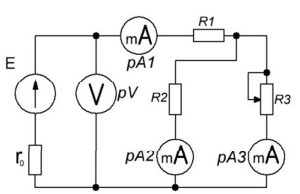
\includegraphics[scale=0.7]{./imgs/ElectricCircuit2.jpg}
		\end{center}
		
		\FPeval{\REtotal}{clip(\ROne + \RTwo * \RMax / (\RTwo + \RMax))}
		\FPround{\REtotal}{\REtotal}{2}
		\[
			R_E = R_1 + \frac{R_2 R_3}{R_2 + R_3} = \ROne + \frac{\RTwo \cdot \RMax}{\RTwo + \RMax} = \REtotal \ \Omega
		\]

		\FPeval{\IExTwoCalcOne}{clip(15 / \REtotal * 1000)}
		\FPround{\IExTwoCalcOne}{\IExTwoCalcOne}{2}

		\[
			I_1 = \frac{E}{r_0 + R_E} = \frac{15}{0 + \REtotal} = \IExTwoCalcOne \ mA
		\]

		\FPeval{\UExTwoCalcTwo}{clip(\IExTwoCalcOne * \RTwo * \RMax / (\RTwo + \RMax) / 1000)}
		\FPround{\UExTwoCalcTwo}{\UExTwoCalcTwo}{2}

		\[
			U_2 = U_3 = I_1 \frac{R_2 R_3}{R_2 + R_3} =
				\IExTwoCalcOne \cdot \frac{\RTwo \cdot \RMax}{\RTwo + \RMax} =
				\UExTwoCalcTwo \ V
		\]

		\FPeval{\UExTwoCalcOne}{clip(\IExTwoOne * \ROne / 1000)}
		\FPround{\UExTwoCalcOne}{\UExTwoCalcOne}{2}

		\[
			U_1 = I_1 \cdot R_1 = \IExTwoOne \cdot \ROne = \UExTwoCalcOne \ V
		\]

		\FPeval{\IExTwoCalcTwo}{clip(\UExTwoCalcTwo / \RTwo * 1000)}
		\FPround{\IExTwoCalcTwo}{\IExTwoCalcTwo}{2}

		\[
			I_2 = \frac{U_2}{R_2} = \frac{\UExTwoCalcTwo}{\RTwo} = \IExTwoCalcTwo \ mA
		\]

		\FPeval{\IExTwoCalcThree}{clip(\UExTwoCalcTwo / \RMax * 1000)}
		\FPround{\IExTwoCalcThree}{\IExTwoCalcThree}{2}

		\[
			I_3 = \frac{U_3}{R_3} = \frac{\UExTwoCalcTwo}{\RMax} = \IExTwoCalcThree \ mA
		\]


		\begin{center} \begin{tabular}{|c|c|c|c|c|c|c|c|c|c|}
			\hline
				\multicolumn{2}{|c|}{R ($\Omega$)} &
				\multicolumn{2}{c|}{$I_c (mA)$} &
				\multicolumn{2}{c|}{$U_c (V)$} &
				\multicolumn{2}{c|}{$I_m (mA)$} &
				\multicolumn{2}{c|}{$U_m (V)$}\\
			\hline

			$R_1$ & \ROne & $I_1$ & \IExTwoCalcOne & $U_1$ & \UExTwoCalcOne & $I_1$ & \IExTwoOne & $U_1$ & \UExTwoOne\\
			\hline

			$R_2$ & \RTwo & $I_2$ & \IExTwoCalcTwo & $U_2$ & \UExTwoCalcTwo & $I_2$ & \IExTwoTwo & $U_2$ & \UExTwoTwo\\
			\hline

			$R_3$ & \RMax & $I_3$ & \IExTwoCalcThree & $U_3$ & \UExTwoCalcTwo & $I_3$ & \IExTwoThree & $U_3$ & \UExTwoThree\\
			\hline
		\end{tabular} \end{center}

\end{document}
